\section{Preliminary Evaluation}

We built a FUSE-based middleware filesystem prototype and tested it on a
64-node cluster with dual core machines with 16GB memory interconnected with a 
GigE NIC.
Each node had a \giga{} indexing server process that managed its own \ldb instance 
that was stored on a local disk running Linux Ext3 file system.
To emulate the shared storage in cluster file systems, we used a NFS-mounted
volume that was accessible from all machines; this volume was used to 
test our cross-server \ldb split optimization.
We evaluated the performance of a single-node \ldb-based metadata store and
the scalability of our distributed middleware.

We first evaluated the performance of a single-node \ldb-based metadata store
by running a test that creates 100 million zero-length files in a single
directory.
%To see the scalability of \ldb-based metadata store for supporting large directories,
%we run a test that creates 100 million zero-length files in a single directory,
Figure \ref{graph:ldb-singlenode} compares the instantaneous throughput of \ldb-based metadata 
store with three Linux file systems: Ext4 \citep{Ext4}, XFS \citep{XFS}, and
Btrfs \citep{BTRFS}.
%Figure \ref{graph:ldb-singlenode} shows a throughput timeline during the test. 
All systems perform well at the beginning of the test, but the file create
throughput drops gradually for all systems. 
Btrfs suffers the most serious throughput drop, slowing down to 100 operations 
per second. However, the \ldb-based store maintains a more steady performance 
with an average speed of 2,200 operations per second respectively,
\textit{and is 10X faster than all other tested file systems.}

\begin{figure}[t]  %%%%%%%%%%%%%%%%%%%%%%%
\centerline{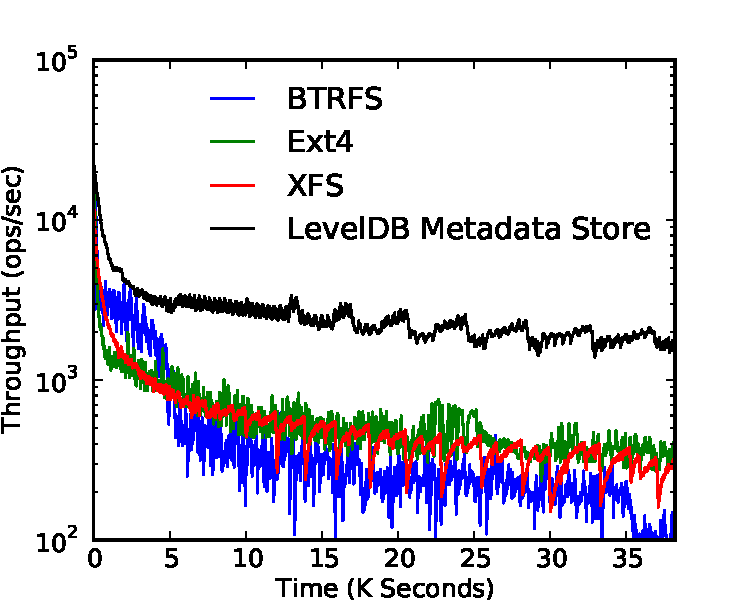
\includegraphics[scale=0.45]{./figs/ldb_insertrate_onenode}}
\caption{
{\small 
Single-node \ldb{}-based metadata store is 10X faster than modern Linux
filesystems for a workload that creates 100 million zero-length files.
X-axis only shows the time until LevelDB finished all insertions because the other 
file systems were much slower. Y-axis is in logarithmic scale.
}
}
\vspace{15pt}
\hrule 
\label{graph:ldb-singlenode}
\end{figure}       %%%%%%%%%%%%%%%%%%%%%%%


Next, we evaluated the scalability of our distributed metadata middleware.
Figure \ref{graph:ldb-scaling} shows the instantaneous throughput during the 
\textit{concurrent create} workload in a strong scaling experiment, i.e.
creating 1 million files per server and reaching up to 64 million files in the
64 server configuration.
The main result in this figure is that as the number of servers doubles the
throughput of the system also scales up. With 64 servers, \giga{} can achieve a
peak throughput of about 190,000 file creates per second. The system delivers
this peak performance after the directory workload has been spread among all
servers.
Before reaching steady-state, the throughput grows gradually due to the splitting
policies adopted by \giga{}.
 
Another observation in Figure \ref{graph:ldb-scaling} is that the system is
unable to sustain the steady-state peak throughput (similar to our observation
in the single-node test in Figure \ref{graph:ldb-singlenode}): 
in fact, in large setups with 8 or more servers, 
the peak throughput drops by as much as 25\% (in case of the 64-server setup).
This is because when there are more entries already existing in \ldb, 
it requires more work to make \ldb balance when inserting a new entry.
In theory, the work of inserting a new entry to a LSM-tree is $O(\log_{B}(n))$
where $n$ is the total number of inserted entries, and $B$ is a constant factor
proportional to the average number of entries transferred in each disk request. 
Thus we can use the formula $\frac{a\cdot S+b}{\log{T}}$ to approximate the 
throughput timelines in Figure \ref{graph:ldb-scaling}, where $S$ is the number 
of servers, $T$ is the time, and $a$ as well as $b$ are constant factors relative 
to the disk speed and splitting overhead.
This estimation shows that when inserting 64 \textit{billion} files into 64 
servers, the system can deliver about 1,000 operations per second per server -- 
64,000 operations in aggregate. 

\begin{figure}[t]  %%%%%%%%%%%%%%%%%%%%%%%
\centerline{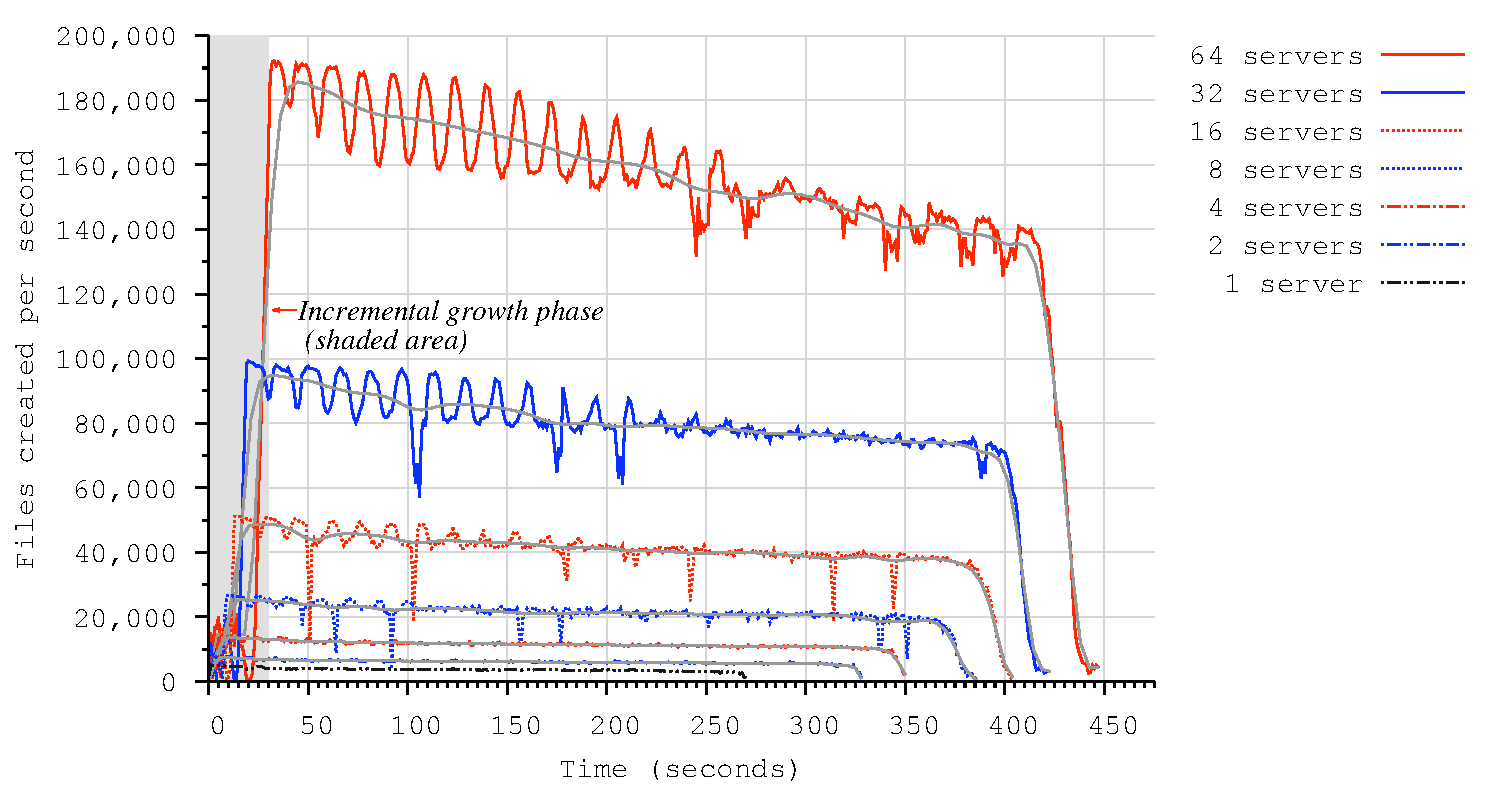
\includegraphics[scale=0.33]{./figs/ldb_insertrate}}
\caption{
{\small
Our middleware metadata service prototype shows promising scalability
up to 64 servers. However the interaction between LevelDB's compaction policies and 
the Linux Ext3's implementation policies causes periodic throughput variance
that degrades as the the number of directory entries in each LevelDB
increases. \textit{Note that the solid lines in each configuration are Bezier
curves to smooth the variability.}
}
}
\vspace{15pt}
\hrule 
\label{graph:ldb-scaling}
\end{figure}       %%%%%%%%%%%%%%%%%%%%%%%

